% Description : Master file of notes building with LaTex Traditional.
% -*- coding:utf-8 -*-
% Author : Wang Jianzhao
% Date : 2020-02-19
% ==================================================================================================================

\documentclass[11pt, a4paper]{article}

% Page Setup
	\usepackage{geometry}
	\geometry{left=3.17cm,right=3.17cm,top=2.54cm,bottom=2.54cm}
	% \setlength{\parindent}{0pt} % Set no indent this article.
	\usepackage{indentfirst}    % Set first paragraph indent.
	% \setlength{\parskip}{1em}   % Set paragraph space.
	% \setlength{\lineskip}{2em}  % Set line space.

% Header and Footer
	\usepackage{fancyhdr}
	\pagestyle{fancy}
	\lhead{Author}
	\chead{Input your title here.}
	\rhead{\thepage}
	\cfoot{}

% Packages may be used
	\usepackage{xcolor}
	\usepackage{amssymb}
	\usepackage{setspace}
	\usepackage{graphicx}
	\usepackage{subfigure}
	\usepackage{caption}
	\usepackage{subfig}
	% \usepackage[colorlinks, citecolor=blue]{hyperref}
	\usepackage{amsmath}
	\numberwithin{equation}{section} % Set equations number style.

\newcommand{\tcr}{\textcolor{blue}}
\newcommand{\upcite}[1]{\textsuperscript{\textsuperscript{\tcr{\cite{#1}}}}}

\title{{\Huge Input your title here}}
\author{Your name}

\begin{document}
\maketitle

\tableofcontents

\newpage
% \begin{center}
% \section{Section 1}
% \end{center}
% \vspace{3ex}
% \begin{spacing}{2.0}

\section{Section One}

Text\upcite{ref1}.

Text\cite{ref1,ref2}.

Text.

\section{Section Two}

Text.

\subsection{Paragraph One}

Figures.

\begin{figure}[h]
	\centering
	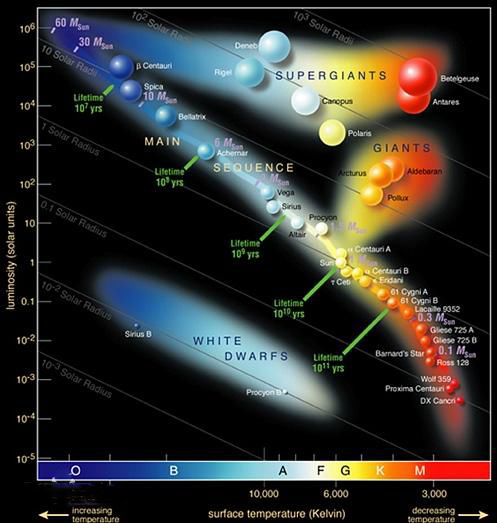
\includegraphics[width=4cm,height=5cm]{2-1.png}
	\caption{This is Figure 1.}
\end{figure}

\begin{figure}[ht]
	\centering
	\subfigure[Figure 2(a)]{
	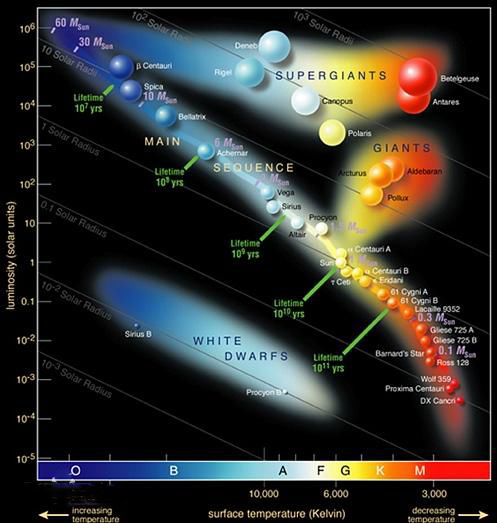
\includegraphics[width=4cm,height=5cm]{2-1.png}}
	\hspace{0in}
	\subfigure[Figure 2(b)]{
	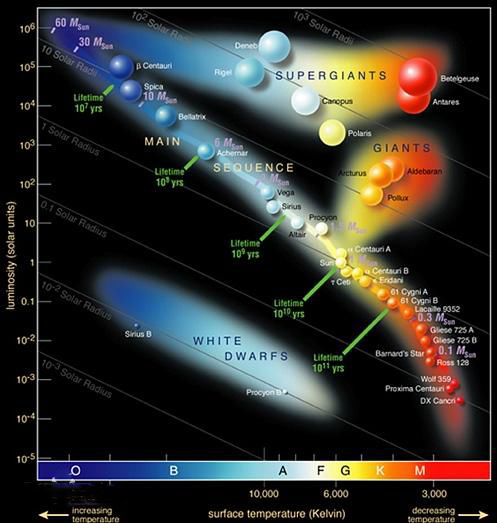
\includegraphics[width=4cm,height=5cm]{2-1.png}}
	\caption{This is Figure 2.}
\end{figure}

\subsection{Paragraph Two}

Equations.

\begin{equation}
	\mathbf{E}=\sum_{l=0}^{\infty} \sum_{m=-l}^{l}\left(E_{l m}^{r}(r) \mathbf{Y}_{l m}+E_{l m}^{(1)}(r) \mathbf{\Psi}_{l m}+E_{l m}^{(2)}(r) \mathbf{\Phi}_{l m}\right)
\end{equation}

\begin{align}
	\mathbf{Y}_{l m}    & =Y_{l m}(\phi,\theta)\  \hat{\mathbf{e}}_r \\
    \mathbf{\Psi}_{l m} & =r \nabla Y_{l m}=\frac{1}{\sin \theta} \frac{\partial Y_{lm}}{\partial \phi}\hat{\mathbf{e}_{\phi}} + \frac{\partial Y_{lm}}{\partial \theta}\hat{\mathbf{e}_{\theta}} \\
    \notag
    \mathbf{\Phi}_{l m} & =\overrightarrow{\mathbf{r}} \times \nabla Y_{l m}=\frac{\partial Y_{lm}}{\partial \theta}\hat{\mathbf{e}_{\phi}} -\frac{1}{\sin \theta} \frac{\partial Y_{lm}}{\partial \phi}\hat{\mathbf{e}_{\theta}}
\end{align}

\subsection{Paragraph Three}

Tables.

\begin{table}[h]
	\renewcommand\arraystretch{2}
	\centering
	\caption{This is table 1.}
	\begin{tabular}{|c|c|c|c|}
		\hline \        & X & Y             & Z             \\
		\hline particle & 2 & $\frac{3}{4}$ & $\frac{1}{2}$ \\
		\hline ion      & 1 & $\frac{1}{4}$ & 0             \\
		\hline electron & 1 & $\frac{2}{4}$ & $\frac{1}{2}$ \\
		\hline
	\end{tabular}
\end{table}

\section{Section Three}

Reference.

\begin{thebibliography}{99}  
\bibitem{ref1}Zheng L, Wang S, Tian L, et al., ApJ, 2015: 1741-1750.  
\bibitem{ref2}Arandjelov R, Zisserman A, IEEE, 2012: 2911-2918.  
\end{thebibliography}

% \end{spacing}

\end{document}
